\section{Realna števila}

\begin{frame}
    \sectionpage
\end{frame}

\begin{frame}
    \tableofcontents[currentsection, hideothersubsections]
\end{frame}

    \subsection{Realna števila}

        \begin{frame}
            \frametitle{Realna števila}

            \only<2->{\begin{block}{}
                Med poljubnima dvema racionalnima številoma $\frac{x}{y}, \frac{z}{w}\in\mathbb{Q}$ je vsaj še eno racionalno število
                 \only<3->{-- aritmetična sredina teh dveh števil $\frac{1}{2}\left(\frac{x}{y}+\frac{z}{w}\right)$.}
            \end{block}}

            \only<4->{\begin{block}{}
                $$\dfrac{x}{y}<\dfrac{z}{w},\ y,w\neq 0 \quad \Rightarrow \quad \dfrac{x}{y}<\frac{1}{2}\left(\dfrac{x}{y}+\dfrac{z}{w}\right)<\dfrac{z}{w}$$
            \end{block}}

            \only<5->{\begin{alertblock}{}
                Med poljubnima racionalnima številoma je neskončno mnogo racionalnih števil in pravimo, da je množica $\mathbb{Q}$ \textbf{povsod gosta}. 
            \end{alertblock}}

            \only<6->{\begin{block}{}
                Množici $\mathbb{Q}$ in $\mathbb{Z}$ imata enako moč -- sta števno neskončni ($m(\mathbb{Q})=m(\mathbb{Z})=\aleph_0$).
            \end{block}}
        \end{frame}


        \begin{frame}
            \only<2->{\begin{alertblock}{Iracionalna števila}
                \only<3->{\textbf{Iracionalna števila} $\mathbb{I}$ so vsi kvadratni koreni števil, ki niso popolni kvadrati, tretji koreni, ki niso popolni kubi, ..., 
                število $\pi$, Eulerjevo število $e$ ... }
            \end{alertblock}}

            \only<4->{\begin{block}{}
                Množici racionalnih in iracionalnih števil sta disjunktni: $\mathbb{Q}\cap\mathbb{I}=\emptyset$.
            \end{block}}

            \only<5->{\begin{alertblock}{Realna števila}
                \only<6->{\textbf{Realna števila} so množica števil, ki jo dobimo kot unijo racionalnih in iracionalnih števil: $\mathbb{R}=\mathbb{Q}\cup\mathbb{I}$.}
            \end{alertblock}}

            \only<7->{\begin{block}{}
                Množica realnih števil je močnejša od množice racionalnih števil. Pravimo, da je (neštevno) neskončna.
            \end{block}}

        \end{frame}


        \begin{frame}

            \only<2->{\begin{block}{}
                Množico realnih števil lahko, glede na predznak števil, razdelimo na tri množice:
                \begin{itemize}
                    \item<3-> \textcolor{green}{množico negativnih realnih števil $\mathbf{\mathbb{R}^-}$},
                    \item<4-> množico z elementom nič: $\mathbf{\{0\}}$ in
                    \item<5-> \textcolor{red}{množico pozitivnih realnih števil: $\mathbf{\mathbb{R}^+}$}.
                \end{itemize}
                $$ \mathbb{R}=\only<3->{\textcolor{green}{\mathbb{R}^-}}\only<4->{\cup\{0\}}\only<5->{\cup\textcolor{red}{\mathbb{R}^+}} $$
            \end{block}}

            \only<2->{\begin{block}{}
                \centering
                \begin{tikzpicture}
                    % \clip (0,0) rectangle (14.000000,10.000000);
                    {\footnotesize
                    
                    % Drawing segment A B
                    \draw [line width=0.016cm] (1.000000,1.500000) -- (4.460000,1.500000);%
                    \draw [line width=0.016cm] (4.540000,1.500000) -- (8.000000,1.500000);%
                    
                    % Marking point 0 by circle
                    \draw [line width=0.016cm] (4.500000,1.500000) circle (0.040000);%
                    \draw (4.500000,1.500000) node [anchor=south] { $0$ };%
                    
                    \only<5->{
                    % Changing color 255 0 0
                    \definecolor{r255g0b0}{rgb}{1.000000,0.000000,0.000000}%
                    \color{r255g0b0}% 
                    
                    % Marking point \mathbb{Q}^+
                    \draw (6.250000,1.500000) node [anchor=south] { $\mathbb{R}^+$ };%
                    
                    % Drawing segment B 0
                    \draw [line width=0.016cm] (8.000000,1.500000) -- (4.540000,1.500000);%
                    }

                    \only<3->{
                    % Changing color 0 255 0
                    \definecolor{r0g255b0}{rgb}{0.000000,1.000000,0.000000}%
                    \color{r0g255b0}% 
                    
                    % Marking point \mathbb{Q}^-
                    \draw (2.750000,1.500000) node [anchor=south] { $\mathbb{R}^-$ };%
                    
                    % Drawing segment A 0
                    \draw [line width=0.016cm] (1.000000,1.500000) -- (4.460000,1.500000);%
                    }

                    % Changing color 0 0 0
                    \definecolor{r0g0b0}{rgb}{0.000000,0.000000,0.000000}%
                    \color{r0g0b0}% 
                    
                    % Marking point \mathbb{Q}
                    \draw (1.500000,2.000000) node  { $\mathbb{R}$ };%
                    \color{black}
                    }
                    \end{tikzpicture}
                    
            \end{block}}

            
            \only<6->{\begin{block}{}
                Vsaki točki na številski premici ustreza natanko eno realno število in obratno, 
                vsakemu realnemu številu ustreza natanko ena točka na številski premici.
            \end{block}}

            \only<7->{\begin{block}{}
                Številsko premico, ki upodablja realna števila, imenujemo tudi \textbf{realna os}.
            \end{block}}


        \end{frame}


        \begin{frame}
            \only<2->{\begin{alertblock}{}
                Z relacijo \textit{biti manjši ali enak} je množica $\mathbb{R}$ \textbf{linearno urejena}, 
                to pomeni, da veljajo:

                \begin{itemize}
                    \item<3-> \textbf{refleksivnost}: \only<4->{$\forall x\in\mathbb{R}: x\leq x$;}
                    \item<5-> \textbf{antisimetričnost}: \only<6->{$\forall x,y\in\mathbb{R}: x\leq y \land y\leq x \Rightarrow x=y$;}
                    \item<7-> \textbf{tranzitivnost}: \only<8->{$\forall x,y,z\in\mathbb{R}: x\leq y \land y\leq z \Rightarrow x\leq z$;}
                    \item<9-> \textbf{stroga sovisnost}: \only<10->{$\forall x,y\in\mathbb{R}: x\leq y \lor y\leq x$.}
                \end{itemize}
            \end{alertblock}}


            \only<11->{\begin{block}{}
                Za realcijo urejenosti na množici $\mathbb{R}$ veljajo še naslednje lastnosti:

                \begin{itemize}
                    \item<12-> \textbf{monotonost vsote}: \only<13->{$x<y \Rightarrow x+z<y+z$ oziroma $x\leq y \Rightarrow x+z\leq y+z$;}
                    \item<14-> $x<y \land z>0 \Rightarrow xz<yz$ in $x\leq y \land z>0 \Rightarrow x z\leq y z$;
                    \item<15-> $x<y \land z<0 \Rightarrow xz>yz$ in $x\leq y \land z<0 \Rightarrow x z\geq y z$.
                \end{itemize}

            \end{block}}

        \end{frame}


        %%%% kvadratni koren 

    \subsection{Kvadratni koren}

        \begin{frame}
            \frametitle{Kvadratni koren}

            \only<2->{\begin{alertblock}{}
                \textbf{Kvadratni koren} $\sqrt{a}$ realnega števila $a\geq 0$ je tisto nenegativno realno število $x$,
                katerega kvadrat je enak $a$.
                \only<3->{$$\sqrt{a}=x \Leftrightarrow a=x^2; \quad a,x\in\mathbb{R}^+ $$}

                \only<4->{Število $a$ imenujemo \textbf{korenjenec}, simbol $\sqrt{~}$ pa \textbf{korenski znak}.}
            \end{alertblock}}

            \only<5->{\begin{block}{Pravila za računanje s kvadratnimi koreni}
                    \begin{columns}
                    \column{0.45\textwidth}
                        \only<6->{\begin{itemize}
                            \item<6-> $\left(\sqrt{a}\right)^2=a; ~a\geq 0$
                            \item<7-> $\sqrt{a^2}=\begin{cases}
                                a, & a\geq 0 \\
                                -a, & a<0
                            \end{cases}$
                        \end{itemize}}
                    \column{0.45\textwidth}
                        \only<8->{\begin{itemize}
                            \item<8-> $\sqrt{a\cdot b}=\sqrt{a}\cdot\sqrt{b}; ~a,b\geq 0$
                            \item<9-> $\sqrt{\dfrac{a}{b}}=\dfrac{\sqrt{a}}{\sqrt{b}}; ~a\geq 0, b>0$
                        \end{itemize}}
                    \end{columns}
            \end{block}}

        \end{frame}

        \begin{frame}
            \only<2->{\begin{block}{Delno korenjenje}
                \only<3->{\textbf{Delno korenjenje} poteka tako, da korenjenec zapišemo kot produkt dveh ali več faktorjev,
                od katerih je vsaj en popoln kvadrat (ga lahko korenimo).
                
                Nato koren zapišemo kot produkt korenov in korenimo kar lahko.}
                \only<4->{$$\sqrt{a^2b}=\sqrt{a^2}\sqrt{b}=a\sqrt{b}$$}
            \end{block}}

            \only<5->{\begin{block}{Racionalizacija imenovalca}
                \only<6->{\textbf{Racionalizacija imenovalca} pomeni, da ulomek zapišemo z enakovrednim ulomkom, ki v imenovalcu nima korena.
                To naredimo z razširjanjem ulomka.}
            \end{block}}

            \only<7->{\begin{block}{}
                Izraze s kvadratnimi koreni poenostavimo tako, da uporabimo že znane obrazce, delno korenimo in racionaliziramo imenovalce.
            \end{block}}
        \end{frame}

        %%% naloge

        \begin{frame}
            \only<2->{\begin{exampleblock}{Naloga}
                Izračunajte.
                \only<3->{\begin{itemize}
                    \begin{columns}
                        \column{0.4\textwidth}
                        \item $\sqrt{49\cdot 64}$ \\~
                        \item $\sqrt{4\cdot 324}$ \\~
                        \item $\sqrt{361\cdot 16}$ \\~
                        \item $\sqrt{-16\cdot 25}$ \\~
                        \item $\sqrt{3\cdot 12}$ \\~
                        \column{0.4\textwidth}
                        \item $\sqrt{\dfrac{225}{289}}$ \\~
                        \item $\sqrt{\dfrac{169}{256}}$ \\~
                        \item $\sqrt{\dfrac{49}{121}}$ \\~
                        \item $\sqrt{\dfrac{18}{32}}$ \\~
                    \end{columns}

                \end{itemize}}
            \end{exampleblock}}
        \end{frame}

        \begin{frame}
            \only<2->{\begin{exampleblock}{Naloga}
                Izračunajte.
                \only<3->{\begin{itemize}
                        \item $\sqrt{\sqrt{16}}$ \\~
                        \item $\sqrt{\sqrt{81}}$ \\~
                        \item $\sqrt{\sqrt{256}}$ \\~
                        \item $\sqrt{\sqrt{1}}$ \\~
                        \item $\sqrt{\sqrt{\sqrt{256}}}$ \\~
                \end{itemize}}
            \end{exampleblock}}
        \end{frame}

        \begin{frame}
            \only<2->{\begin{exampleblock}{Naloga}
                Izračunajte.
                \only<3->{\begin{itemize}
                        \item $\sqrt{x^4y^8}$ \\~
                        \item $\sqrt{e^{10}f^{26}}$ \\~
                        \item $\sqrt{a^{20}b^4}$ \\~
                        \item $\sqrt{(-x)^{20}y^4}$ \\~
                        \item $\sqrt{3a^6+a^6}$ \\~
                \end{itemize}}
            \end{exampleblock}}
        \end{frame}


        \begin{frame}
            \only<2->{\begin{exampleblock}{Naloga}
                Izračunajte.
                \only<3->{\begin{itemize}
                    \begin{columns}
                        \column{0.4\textwidth}
                        \item $\sqrt{16+36+12}$ \\~
                        \item $\sqrt{121}+\sqrt{81}$ \\~
                        \item $\sqrt{10+21+69}$ \\~
                        \item $\sqrt{10+11-21}$ \\~
                        \item $\sqrt{9+4-4}$ \\~
                        \column{0.4\textwidth}
                        \item $\sqrt{3\cdot 4+2\cdot 2}$ \\~
                        \item $\sqrt{5\cdot 7 +1}$ \\~
                        \item $\sqrt{8\cdot 7-5\cdot 4}$ \\~
                        \item $\sqrt{10\cdot 8-4\cdot 4}$ \\~
                        \item $\sqrt{11\cdot 5+2\cdot 7+3\cdot 4}$ \\~
                    \end{columns}

                \end{itemize}}
            \end{exampleblock}}
        \end{frame}

        \begin{frame}
            \only<2->{\begin{exampleblock}{Naloga}
                Izračunajte.
                \only<3->{\begin{itemize}
                    \begin{columns}
                        \column{0.4\textwidth}
                        \item $\sqrt{20}$ \\~
                        \item $\sqrt{98}$ \\~
                        \item $\sqrt{300}$ \\~
                        \item $\sqrt{125}$ \\~
                        \item $\sqrt{x^3}$ \\~
                        \column{0.4\textwidth}
                        \item $\sqrt{x^4y^5z^6}$ \\~
                        \item $\sqrt{128a^{13}b^9}$ \\~
                        \item $\sqrt{100x^2y^5+62x^2y^5}; \quad x,y\geq 0$ \\~
                        \item $\sqrt{8a^6b^5-12a^4b^6}; \quad a,b\geq 0$ \\~
                    \end{columns}

                \end{itemize}}
            \end{exampleblock}}
        \end{frame}


        \begin{frame}
            \only<2->{\begin{exampleblock}{Naloga}
                Izračunajte.
                \only<3->{\begin{itemize}
                        \item $\sqrt{44}+\sqrt{99}$ \\~
                        \item $\sqrt{192}+\sqrt{147}$ \\~
                        \item $\sqrt{180}-\sqrt{245}+2\sqrt{500}$ \\~
                        \item $\sqrt{243a^3b}+2a\sqrt{48ab}-\sqrt{363a^2}\cdot\sqrt{ab}; \quad a,b\geq 0$ \\~
                        \item $\sqrt{3a^6+a^6}$ \\~
                \end{itemize}}
            \end{exampleblock}}
        \end{frame}


        \begin{frame}
            \only<2->{\begin{exampleblock}{Naloga}
                Racionalizirajte imenovalec.
                \only<3->{\begin{itemize}
                    \begin{columns}
                        \column{0.4\textwidth}
                        \item $\dfrac{2}{\sqrt{3}}$ \\~\\~
                        \item $\dfrac{2+\sqrt{2}}{\sqrt{2}}$ \\~\\~
                        \item $\dfrac{2}{5\sqrt{3}}$ \\~\\~
                        \column{0.4\textwidth}
                        \item $\dfrac{\sqrt{2}}{1-\sqrt{2}}$ \\~\\~
                        \item $\dfrac{1+\sqrt{5}}{2+\sqrt{5}}$ \\~\\~
                        \item $\dfrac{2-\sqrt{3}}{3+\sqrt{2}}$ \\~\\~
                    \end{columns}

                \end{itemize}}
            \end{exampleblock}}
        \end{frame}


        \begin{frame}
            \only<2->{\begin{exampleblock}{Naloga}
                Izračunajte.
                \only<3->{\begin{itemize}
                    \begin{columns}
                        \column{0.4\textwidth}
                        \item $\dfrac{2}{\sqrt{3}}+\dfrac{3}{\sqrt{2}}$ \\~\\~\\~
                        \item $\dfrac{1-\sqrt{2}}{\sqrt{3}}-\dfrac{\sqrt{2}}{\sqrt{5}}$ \\~\\~
                        \column{0.4\textwidth}
                        \item $\left(1+\sqrt{5}\right)^2$ \\~\\~
                        \item $\left(3-\sqrt{2}\right)^2$ \\~\\~
                        \item $\left(2-\sqrt{3}\right)^3$ \\~\\~
                    \end{columns}

                \end{itemize}}
            \end{exampleblock}}
        \end{frame}


        
        \begin{frame}
            \only<2->{\begin{exampleblock}{Naloga}
                Izračunajte.
                \only<3->{\begin{itemize}
                    \begin{columns}
                        \column{0.4\textwidth}
                        \item $\left(2-\sqrt{5}\right)^3-\left(1+2\sqrt{5}\right)^2$ \\~\\~\\~
                        \item $\left(2-\sqrt{3}\right)^2+\left(2+\sqrt{3}\right)^3$ \\~\\~
                        \column{0.4\textwidth}
                        \item $\left(1+\sqrt{5}\right)\sqrt{6-2\sqrt{5}}$ \\~\\~
                        \item $\left(3-\sqrt{5}\right)\sqrt{14+6\sqrt{5}}$ \\~\\~
                        \item $\left(\sqrt{3}+\sqrt{5}\right)\sqrt{8-2\sqrt{15}}$ \\~\\~
                    \end{columns}

                \end{itemize}}
            \end{exampleblock}}
        \end{frame}


        % \begin{frame}
        %     \only<2->{\begin{exampleblock}{Naloga}
        %         Poenostavite.
        %         \only<3->{\begin{itemize}
        %             \item a \\~
        %         \end{itemize}}
        %     \end{exampleblock}}
        % \end{frame}


        % \begin{frame}
        %     \only<2->{\begin{exampleblock}{Naloga}
        %         Poenostavite.
        %         \only<3->{\begin{itemize}
        %             \item a \\~
        %         \end{itemize}}
        %     \end{exampleblock}}
        % \end{frame}


        % \begin{frame}
        %     \only<2->{\begin{exampleblock}{Naloga}
        %         Poenostavite.
        %         \only<3->{\begin{itemize}
        %             \item a \\~
        %         \end{itemize}}
        %     \end{exampleblock}}
        % \end{frame}

    \subsection{Kubični koren}

        \begin{frame}
            \frametitle{Kubični koren}

            \only<2->{\begin{alertblock}{}
                \textbf{Kubični koren} $\sqrt[3]{a}$ realnega števila $a$ je tisto realno število $x$,
                katerega kub je enak $a$.
                \only<3->{$$\sqrt[3]{a}=x \Leftrightarrow a=x^3; \quad a,x\in\mathbb{R}$$}

                \only<4->{Število $a$ imenujemo \textbf{korenjenec}, simbol $\sqrt{~}$ \textbf{korenski znak}, število $3$ pa \textbf{korenski eksponent}.}
            \end{alertblock}}

            \only<5->{\begin{block}{Pravila za računanje s kubičnimi koreni}
                \begin{columns}
                \column{0.44\textwidth}
                    \only<5->{\begin{itemize}
                        \item<6-> $\left(\sqrt[3]{a}\right)^3=a$
                        \item<7-> $\sqrt[3]{a^3}=a$
                    \end{itemize}}
                \column{0.44\textwidth}
                    \only<8->{\begin{itemize}
                        \item<8-> $\sqrt[3]{a\cdot b}=\sqrt[3]{a}\cdot\sqrt[3]{b}$
                        \item<9-> $\sqrt[3]{\dfrac{a}{b}}=\dfrac{\sqrt[3]{a}}{\sqrt[3]{b}}; ~b\neq 0$
                    \end{itemize}}
                \end{columns}
            \end{block}}

        \end{frame}


        \begin{frame}
            \only<2->{\begin{exampleblock}{Naloga}
                Izračunajte.
                \only<3->{\begin{itemize}
                    \begin{columns}
                        \column{0.4\textwidth}
                        \item $\sqrt[3]{-1}$ \\~\\~
                        \item $\sqrt[3]{216}$ \\~\\~
                        \item $\sqrt[3]{8}$ \\~\\~
                        \column{0.4\textwidth}
                        \item $\sqrt[3]{\dfrac{64}{125}}$ \\~\\~
                        \item $\sqrt[3]{-\dfrac{27}{343}}$ \\~\\~
                        \item $\sqrt[3]{1\dfrac{488}{512}}$ \\~\\~
                    \end{columns}

                \end{itemize}}
            \end{exampleblock}}
        \end{frame}


        \begin{frame}
            \only<2->{\begin{exampleblock}{Naloga}
                Izračunajte.
                \only<3->{\begin{itemize}
                        \item $\sqrt{\sqrt{256}}-\dfrac{3-\sqrt{2}}{\sqrt{2}-1}+\sqrt[3]{-8}+\left(2-\sqrt{2}\right)^2$ \\~\\~
                        \item $\dfrac{\sqrt{3}+1}{\sqrt{3}}-\dfrac{\sqrt{3}-1}{\sqrt{3}+1}+\sqrt{0.16}+\sqrt{0.64}-\sqrt[3]{-27}+\sqrt{48}-\sqrt{27}$ \\~\\~
                        \item $\left(1-\sqrt{5}\right)^2-\left(1+\sqrt{5}\right)^2+\dfrac{\sqrt{5}-2}{\sqrt{5}+2}-\sqrt{125}+\sqrt{245}$ \\~\\~
                \end{itemize}}
            \end{exampleblock}}
        \end{frame}

        % \begin{frame}
        %     \begin{exampleblock}{Naloga 563}
        %         Izračunaj in rezultat delno koreni.
        %         \begin{description}
        %             \item<2->[(b)] $\displaystyle 4\sqrt{8}-\left(2\sqrt{5}+3\sqrt{8}\right)\sqrt{10}$
        %             \item<3->[(č)] $\displaystyle\left(5\sqrt{3}+2\sqrt{27}\right)\left(\sqrt{75}-4\sqrt{12}+\sqrt{147}\right)$
        %             \item<4->[(g)] $\displaystyle 8\sqrt{3}\left(\sqrt{2}-1\right)-\left(\sqrt{5}+2\sqrt{6}\right)\left(4-2\sqrt{2}\right)$  
        %             \item<5->[(j)] $\displaystyle\left(2-4\sqrt{3}\right)\cdot 3\sqrt{2}-\left(2\sqrt{2}-3\sqrt{3}\right)^2$
        %             \item<6->[(l)] $\displaystyle\left(3-2\sqrt{2}\right)^3-\left(\sqrt{8}-5\sqrt{2}\right)\left(-3\sqrt{2}\right)$
        %             \item<7->[(o)] $\displaystyle\sqrt{300}-\sqrt{5-2\sqrt{6}}\cdot\sqrt{5+2\sqrt{6}}+\sqrt{5^4}$
        %             \item<8->[(r)] $\displaystyle\sqrt{5\sqrt{3}-5}\cdot\sqrt{2\sqrt{3}+2}-\left(\sqrt{5}\right)^3$  
        %             \item<9->[(u)] $\displaystyle\left(\sqrt{17}-3\right)\sqrt{26+6\sqrt{17}}-\sqrt{2}\left(\sqrt{2}+\sqrt{6}\right)$
        %         \end{description}
        %     \end{exampleblock}
        % \end{frame}

    \subsection{Interval}

        \begin{frame}
            \frametitle{Interval}

            \only<2->{\begin{alertblock}{}
                \textbf{Interval} je množica vseh realnih števil, ki ležijo med dvema danima številoma $a$ in $b$, kjer je $a<b$. \\
                Števili $a$ in $b$ imenujemo \textbf{krajišči intervala}.                
            \end{alertblock}
            }

            \only<3->{\begin{block}{Vključenost krajišč}
                \begin{itemize}
                    \item<4-> Simbola $"["$ in $"]"$ označujeta krajišče, ki spada k intervalu.
                    \item<5-> Simbola $"("$ in $")"$ označujeta krajišče, ki ne spada k intervalu.
                \end{itemize}
            \end{block}
            }

            \only<6->{\begin{block}{}
                Pri zapisu intervalov moramo biti pozorni na zapis vrstnega reda števil, ki določata krajišči.
                $$[a,b]\neq[b,a]$$
            \end{block}
            }

            \note{
                Ponazoritev krajišča na številski premici:
                \begin{itemize}
                    \item odebeljena pika / črtica -- krajišče spada k intervalu;
                    \item puščica -- krajišče ne spada k intervalu.
                \end{itemize}
            }

        \end{frame}

        \begin{frame}
            \frametitle{\large Vrste intervalov}

            \only<2->{\begin{alertblock}{Zaprti interval}
                \only<3->{$$ \mathbf{[a,b]=\left\{x\in\mathbb{R}; a\leq x\leq b\right\} }$$

                \centering
                    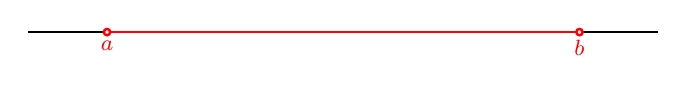
\begin{tikzpicture}
                    % \clip (0,0) rectangle (14.000000,10.000000);
                    {\footnotesize
                    
                    % Drawing line a b
                    \draw [line width=0.016cm] (1.000000,1.500000) -- (1.960000,1.500000);%
                    \draw [line width=0.016cm] (2.040000,1.500000) -- (7.960000,1.500000);%
                    \draw [line width=0.016cm] (8.040000,1.500000) -- (9.000000,1.500000);%
                    
                    % Changing color 255 0 0
                    \definecolor{r255g0b0}{rgb}{1.000000,0.000000,0.000000}%
                    \color{r255g0b0}% 
                    
                    % Drawing segment a b
                    \draw [line width=0.032cm] (2.040000,1.500000) -- (7.960000,1.500000);%
                    
                    % Marking point a by circle
                    \draw [line width=0.032cm] (2.000000,1.500000) circle (0.040000);%
                    \draw (2.000000,1.500000) node [anchor=north] { $a$ };%
                    
                    % Marking point b by circle
                    \draw [line width=0.032cm] (8.000000,1.500000) circle (0.040000);%
                    \draw (8.000000,1.500000) node [anchor=north] { $b$ };%
                    \color{black}
                    }
                    \end{tikzpicture}

                    
                Vsebuje vsa realna števila med $a$ in $b$, vključno s krajiščema $a$ in $b$.
                }
            \end{alertblock}
            }

            \only<4->{\begin{alertblock}{Odprti interval}
                \only<5->{$$ \mathbf{(a,b)=\left\{x\in\mathbb{R}; a<x<b\right\} }$$

                \centering
                    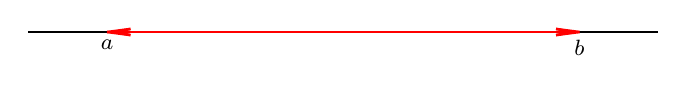
\begin{tikzpicture}
                    % \clip (0,0) rectangle (14.000000,10.000000);
                    {\footnotesize
                    
                    % Drawing line a b
                    \draw [line width=0.016cm] (1.000000,1.500000) -- (9.000000,1.500000);%
                    
                    % Changing color 255 0 0
                    \definecolor{r255g0b0}{rgb}{1.000000,0.000000,0.000000}%
                    \color{r255g0b0}% 
                    
                    % Drawing segment a b
                    \draw [line width=0.032cm] (2.000000,1.500000) -- (8.000000,1.500000);%
                    
                    % Drawing arrow a b 1.00
                    \draw [line width=0.032cm] (7.702567,1.539158) -- (8.000000,1.500000);%
                    \draw [line width=0.032cm] (7.702567,1.539158) -- (7.900856,1.500000);%
                    \draw [line width=0.032cm] (7.702567,1.460842) -- (8.000000,1.500000);%
                    \draw [line width=0.032cm] (7.702567,1.460842) -- (7.900856,1.500000);%
                    
                    % Drawing arrow b a 1.00
                    \draw [line width=0.032cm] (2.297433,1.460842) -- (2.000000,1.500000);%
                    \draw [line width=0.032cm] (2.297433,1.460842) -- (2.099144,1.500000);%
                    \draw [line width=0.032cm] (2.297433,1.539158) -- (2.000000,1.500000);%
                    \draw [line width=0.032cm] (2.297433,1.539158) -- (2.099144,1.500000);%
                    \color{black}
                        
                    % Marking point a
                    \draw (2.000000,1.500000) node [anchor=north] { $a$ };%
                    
                    % Marking point b
                    \draw (8.000000,1.500000) node [anchor=north] { $b$ };%
                    }
                    \end{tikzpicture}
 
                Vsebuje vsa realna števila med $a$ in $b$, vendar ne vsebuje krajišč $a$ in $b$.
                }
            \end{alertblock}
            }

        \end{frame}

        \begin{frame}
            
            \only<2->{\begin{alertblock}{Polodprti/polzaprti interval}
                \begin{itemize}
                    \item<3-> $$ \mathbf{[a,b)=\left\{x\in\mathbb{R}; a\leq x<b\right\} }$$
                    
                    \begin{center}
                        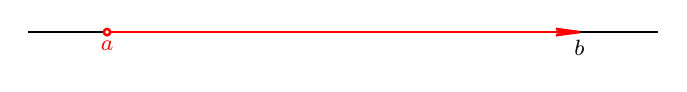
\begin{tikzpicture}
                        % \clip (0,0) rectangle (14.000000,10.000000);
                        {\footnotesize
                        
                        % Drawing line a b
                        \draw [line width=0.016cm] (1.000000,1.500000) -- (1.960000,1.500000);%
                        \draw [line width=0.016cm] (2.040000,1.500000) -- (9.000000,1.500000);%
                        
                        % Changing color 255 0 0
                        \definecolor{r255g0b0}{rgb}{1.000000,0.000000,0.000000}%
                        \color{r255g0b0}% 
                        
                        % Drawing segment a b
                        \draw [line width=0.032cm] (2.040000,1.500000) -- (8.000000,1.500000);%
                        
                        % Marking point a by circle
                        \draw [line width=0.032cm] (2.000000,1.500000) circle (0.040000);%
                        \draw (2.000000,1.500000) node [anchor=north] { $a$ };%
                        
                        % Drawing arrow a b 1.00
                        \draw [line width=0.032cm] (7.702567,1.539158) -- (8.000000,1.500000);%
                        \draw [line width=0.032cm] (7.702567,1.539158) -- (7.900856,1.500000);%
                        \draw [line width=0.032cm] (7.702567,1.460842) -- (8.000000,1.500000);%
                        \draw [line width=0.032cm] (7.702567,1.460842) -- (7.900856,1.500000);%
                        \color{black}
                        
                        % Marking point b
                        \draw (8.000000,1.500000) node [anchor=north] { $b$ };%
                        }
                        \end{tikzpicture}
                    \end{center}

                        
                    Vsebuje vsa realna števila med $a$ in $b$, vključno s krajiščem $a$, vendar ne vsebuje krajišča $b$.
                    

                    \item<4-> $$ \mathbf{(a,b]=\left\{x\in\mathbb{R}; a<x\leq b\right\} }$$
                    
                    \begin{center}
                        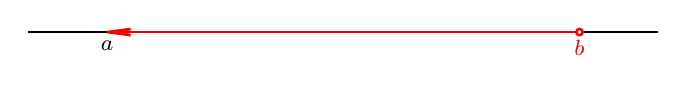
\begin{tikzpicture}
                        % \clip (0,0) rectangle (14.000000,10.000000);
                        {\footnotesize
                        
                        % Drawing line a b
                        \draw [line width=0.016cm] (1.000000,1.500000) -- (7.960000,1.500000);%
                        \draw [line width=0.016cm] (8.040000,1.500000) -- (9.000000,1.500000);%
                        
                        % Changing color 255 0 0
                        \definecolor{r255g0b0}{rgb}{1.000000,0.000000,0.000000}%
                        \color{r255g0b0}% 
                        
                        % Drawing segment a b
                        \draw [line width=0.032cm] (2.000000,1.500000) -- (7.960000,1.500000);%
                        
                        % Marking point b by circle
                        \draw [line width=0.032cm] (8.000000,1.500000) circle (0.040000);%
                        \draw (8.000000,1.500000) node [anchor=north] { $b$ };%
                        
                        % Drawing arrow b a 1.00
                        \draw [line width=0.032cm] (2.297433,1.460842) -- (2.000000,1.500000);%
                        \draw [line width=0.032cm] (2.297433,1.460842) -- (2.099144,1.500000);%
                        \draw [line width=0.032cm] (2.297433,1.539158) -- (2.000000,1.500000);%
                        \draw [line width=0.032cm] (2.297433,1.539158) -- (2.099144,1.500000);%
                        \color{black}

                        % Marking point a
                        \draw (2.000000,1.500000) node [anchor=north] { $a$ };%
                        }
                        \end{tikzpicture}
                    \end{center}

                        
                    Vsebuje vsa realna števila med $a$ in $b$, vključno s krajiščem $b$, vendar ne vsebuje krajišča $a$.

                \end{itemize}


            \end{alertblock}
            }
        \end{frame}

        \begin{frame}
            \only<2->{\begin{alertblock}{Neomejeni/neskončni intervali}
                
                \begin{itemize}
                    \item<3-> $ \mathbf{[a,\infty)=\left\{x\in\mathbb{R}; x\geq a\right\} }$ \\
                    \begin{center}
                        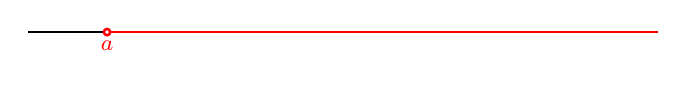
\begin{tikzpicture}
                        % \clip (0,0) rectangle (14.000000,10.000000);
                        {\footnotesize
                        
                        % Drawing line a b
                        \draw [line width=0.016cm] (1.000000,1.500000) -- (1.960000,1.500000);%
                        \draw [line width=0.016cm] (2.040000,1.500000) -- (9.000000,1.500000);%
                        
                        % Changing color 255 0 0
                        \definecolor{r255g0b0}{rgb}{1.000000,0.000000,0.000000}%
                        \color{r255g0b0}% 
                        
                        % Drawing segment a y
                        \draw [line width=0.032cm] (2.040000,1.500000) -- (9.000000,1.500000);%
                        
                        % Marking point a by circle
                        \draw [line width=0.032cm] (2.000000,1.500000) circle (0.040000);%
                        \draw (2.000000,1.500000) node [anchor=north] { $a$ };%
                        \color{black}
                        }
                        \end{tikzpicture}
                    \end{center}
                        
                    \item<4-> $ \mathbf{(a,\infty)=\left\{x\in\mathbb{R}; x>a\right\} }$ \\
                    \begin{center}
                        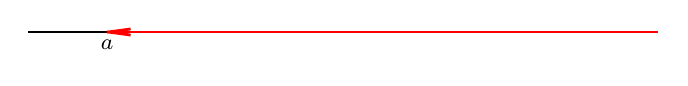
\begin{tikzpicture}
                        % \clip (0,0) rectangle (14.000000,10.000000);
                        {\footnotesize
                        
                        % Drawing line a b
                        \draw [line width=0.016cm] (1.000000,1.500000) -- (9.000000,1.500000);%
                        
                        % Marking point a
                        \draw (2.000000,1.500000) node [anchor=north] { $a$ };%
                        
                        % Changing color 255 0 0
                        \definecolor{r255g0b0}{rgb}{1.000000,0.000000,0.000000}%
                        \color{r255g0b0}% 
                        
                        % Drawing segment a y
                        \draw [line width=0.032cm] (2.000000,1.500000) -- (9.000000,1.500000);%
                        
                        % Drawing arrow b a 1.00
                        \draw [line width=0.032cm] (2.297433,1.460842) -- (2.000000,1.500000);%
                        \draw [line width=0.032cm] (2.297433,1.460842) -- (2.099144,1.500000);%
                        \draw [line width=0.032cm] (2.297433,1.539158) -- (2.000000,1.500000);%
                        \draw [line width=0.032cm] (2.297433,1.539158) -- (2.099144,1.500000);%
                        \color{black}
                        }
                        \end{tikzpicture}
                    \end{center}

                        
                    \item<5-> $\mathbf{(-\infty,b]=\left\{x\in\mathbb{R}; x\leq b\right\} }$ \\
                    \begin{center}
                        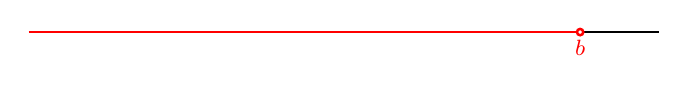
\begin{tikzpicture}
                        % \clip (0,0) rectangle (14.000000,10.000000);
                        {\footnotesize
                        
                        % Drawing line a b
                        \draw [line width=0.016cm] (1.000000,1.500000) -- (7.960000,1.500000);%
                        \draw [line width=0.016cm] (8.040000,1.500000) -- (9.000000,1.500000);%
                        
                        % Changing color 255 0 0
                        \definecolor{r255g0b0}{rgb}{1.000000,0.000000,0.000000}%
                        \color{r255g0b0}% 
                        
                        % Marking point b by circle
                        \draw [line width=0.032cm] (8.000000,1.500000) circle (0.040000);%
                        \draw (8.000000,1.500000) node [anchor=north] { $b$ };%
                        
                        % Drawing segment x b
                        \draw [line width=0.032cm] (1.000000,1.500000) -- (7.960000,1.500000);%
                        \color{black}
                        }
                        \end{tikzpicture}
                    \end{center}

                        
                    \item<6-> $ \mathbf{(-\infty,b)=\left\{x\in\mathbb{R}; x<b\right\} }$ \\
                    \begin{center}
                        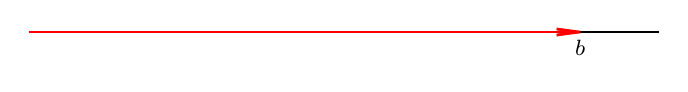
\begin{tikzpicture}
                        % \clip (0,0) rectangle (14.000000,10.000000);
                        {\footnotesize
                        
                        % Drawing line a b
                        \draw [line width=0.016cm] (1.000000,1.500000) -- (9.000000,1.500000);%
                        
                        % Marking point b
                        \draw (8.000000,1.500000) node [anchor=north] { $b$ };%
                        
                        % Changing color 255 0 0
                        \definecolor{r255g0b0}{rgb}{1.000000,0.000000,0.000000}%
                        \color{r255g0b0}% 
                        
                        % Drawing segment x b
                        \draw [line width=0.032cm] (1.000000,1.500000) -- (8.000000,1.500000);%
                        
                        % Drawing arrow a b 1.00
                        \draw [line width=0.032cm] (7.702567,1.539158) -- (8.000000,1.500000);%
                        \draw [line width=0.032cm] (7.702567,1.539158) -- (7.900856,1.500000);%
                        \draw [line width=0.032cm] (7.702567,1.460842) -- (8.000000,1.500000);%
                        \draw [line width=0.032cm] (7.702567,1.460842) -- (7.900856,1.500000);%
                        \color{black}
                        }
                        \end{tikzpicture}
                    \end{center}

                    \item<7-> $ \mathbf{(-\infty,\infty)=\left\{x;x\in\mathbb{R}\right\} =\mathbb{R}}$ \\
                    \begin{center}
                        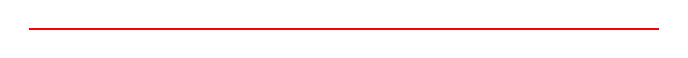
\begin{tikzpicture}
                            % \clip (0,0) rectangle (14.000000,10.000000);
                            {\footnotesize
                            
                            % Drawing line a b
                            \draw [line width=0.016cm] (1.000000,1.500000) -- (9.000000,1.500000);%
                            
                            % Changing color 255 0 0
                            \definecolor{r255g0b0}{rgb}{1.000000,0.000000,0.000000}%
                            \color{r255g0b0}% 
                            
                            % Drawing segment x y
                            \draw [line width=0.032cm] (1.000000,1.500000) -- (9.000000,1.500000);%
                            \color{black}
                            }
                        \end{tikzpicture}
                    \end{center}

                \end{itemize}

            \end{alertblock}
            }

            \note{
                Zapis podmnožic $\mathbb{R}$ z intervali:
            \begin{itemize}
                \item $\mathbb{R}^+=(0,\infty)$
                \item $\mathbb{R}_0^+=[0,\infty)$
                \item $\mathbb{R}^-=(-\infty,0)$
            \end{itemize}
            }
        \end{frame}



        \begin{frame}
            \only<2->{\begin{exampleblock}{Naloga}
                Zapišite kot interval.
                \only<3->{\begin{itemize}
                        \item $\{x\in\mathbb{R}; -2<x<2\}$ \\~\\~
                        \item $\{x\in\mathbb{R}; 4\leq x\leq 2\}$ \\~\\~
                        \item $\{x\in\mathbb{R}; -14<x\leq -9\}$ \\~\\~
                \end{itemize}}
            \end{exampleblock}}
        \end{frame}


        \begin{frame}
            \only<2->{\begin{exampleblock}{Naloga}
                Zapišite interval, ki je narisan na sliki.
                \only<3->{\begin{itemize}
                        \item $ $ \\~\\~
                        \item $ $ \\~\\~
                        \item $ $ \\~\\~
                \end{itemize}}
            \end{exampleblock}}
        \end{frame}


        \begin{frame}
            \only<2->{\begin{exampleblock}{Naloga}
                Zapišite presek intervalov.
                \only<3->{\begin{itemize}
                    \begin{columns}
                        \column{0.4\textwidth}
                        \item $ [0,2)\cap(-1,1]$ \\~\\~
                        \item $ [-3,5]\cap(-3,5)$ \\~\\~
                        \item $ [2,5)\cap[5,7)$ \\~\\~
                        \column{0.4\textwidth}
                        \item $ [-1,3)\cap(-4,-1]$ \\~\\~
                        \item $ [4,6]\cap[-1,4]$ \\~\\~
                        \item $ (-1,3)\cap[1,2)$ \\~\\~
                    \end{columns}

                \end{itemize}}
            \end{exampleblock}}
        \end{frame}


        \begin{frame}
            \only<2->{\begin{exampleblock}{Naloga}
                Zapišite unijo intervalov.
                \only<3->{\begin{itemize}
                        \item $ [0,2)\cup(-1,1]$ \\~\\~
                        \item $ [-3,5]\cup(-3,5)$ \\~\\~
                        \item $ [2,5)\cup[5,7)$ \\~\\~
                        \item $ [-1,3)\cup(-4,1]$ \\~\\~
                \end{itemize}}
            \end{exampleblock}}
        \end{frame}


        
        \begin{frame}
            \only<2->{\begin{exampleblock}{Naloga}
                Zapišite razliko intervalov.
                \only<3->{\begin{itemize}
                        \item $ [2,3]\setminus[3,4)$ \\~\\~
                        \item $ (1,3)\setminus(3,4)$ \\~\\~
                        \item $ [2,5)\setminus(-1,2]$ \\~\\~
                        \item $ (2,8)\setminus[5,6)$ \\~\\~
                \end{itemize}}
            \end{exampleblock}}
        \end{frame}


        \begin{frame}
            \only<2->{\begin{exampleblock}{Naloga}
                Izračunajte.
                \only<3->{\begin{itemize}
                        \item $\left([1,3)\setminus(1,4]\right)\cup(1,2)$ \\~\\~
                        \item $[-2,4]\setminus\left((-1,2]\cap[0,3)\right)$ \\~\\~
                        \item $\left((-2,3]\setminus[-3,2)\right)\cap[3,5)$ \\~\\~
                \end{itemize}}
            \end{exampleblock}}
        \end{frame}


        % \begin{frame}
        %     \only<2->{\begin{exampleblock}{Naloga 423 (Linea nova)}
        %         Zapišite množico vseh neengativnih realnih števil, ki so manjša od $6$, ter iskano množico predstavite na številski premici.
        %     \end{exampleblock}
        %     \note{Rešitev N423: $\left\{x\in\mathbb{R};0\leq x<6 \right\} [0,6)$ \\}
        %     }

        %     \only<3->{\begin{exampleblock}{Naloga 585}
        %         Dana sta intervala $I=[-2,5)$ in $J=(3,6)$.
        %         \begin{itemize}
        %             % \item Intervala $I$ in $J$ nariši na številski premici.
        %             \item<4-> Zapiši $I\cap J$ in $I\cup J$.
        %             \item<5-> Izračunaj vsoto največjega celega števila iz $I$ in najmanjšega celega števila iz $J$.
        %         \end{itemize}
        %     \end{exampleblock}
        %     \note{Rešitev N585:\begin{itemize}
        %         \item $I\cap J=(3,5)$; $I\cup J=[-2,6)$
        %         \item $4+4=8$
        %     \end{itemize} }
        %     }

        %     \only<6->{\begin{exampleblock}{Naloga 583}
        %         Zapiši unijo in presek danih intervalov.
        %         \begin{description}
        %             \item[(c)]<7-> $[4,8]$ in $(3,5]$
        %             \item[(f)]<8-> $[-2,4]$ in $(2,\infty)$
        %             \item[(g)]<9-> $(-\infty,3]$ in $(-1,5]$   
        %         \end{description}
        %     \end{exampleblock}
        %     \note{Rešitev N583: \begin{description}
        %         \item[(c)] $(3,8]$ in $[4,5]$
        %         \item[(f)] $[-2,\infty)$ in $(2,4]$
        %         \item[(g)] $(-\infty,5]$ in $(-1,3]$   
        %     \end{description}
        %     }
        %     }
        % \end{frame}



    \subsection{Reševanje enačb}

        \begin{frame}
            \frametitle{Reševanje enačb}

            \only<2->{\begin{alertblock}{Enačba}
                \only<3->{\textbf{Enačba} je enakost dveh izrazov, pri čemer vsaj v enem nastopa \textbf{neznanka}, ki je ponavadi označena s črko $x$.}

                \only<4->{\textbf{Rešitev enačbe} je vsaka vrednost neznanke, za katero sta vrednosti leve in desne strani enačbe enaki.}
            \end{alertblock}}

            \only<5->{\begin{block}{Reševanje enačbe}
                \only<6->{Enačbo rešujemo tako, da jo preoblikujemo v ekvivalentno enačbo, iz katere preberemo rešitve.}

                \only<7->{Ekvivalentno enačbo dobimo, če:}
                \only<8->{\begin{itemize}
                    \item<8-> na obeh straneh enačbe prištejemo isto število ali izraz;
                    \item<9-> obe strani enačbe množimo z istim neničelnim številom ali izrazom.
                \end{itemize}}
            \end{block}}
        \end{frame}

        \begin{frame}
            \only<2->{\begin{alertblock}{Linearna enačba}
                \only<3->{\textbf{Linearna enačba} je enačba oblike $ax+b=0;~a,b\in\mathbb{R}$.}

                \only<4->{Rešujemo jo tako, da jo preoblikujemo v ekvivalentno enačbo, ki ima na eni strani samo neznanko.}
            \end{alertblock}}

            \only<5->{\begin{alertblock}{Razcepna enačba}
                \only<6->{\textbf{Razcepna enačba} je enačba, v kateri nastopajo potence neznanke (na primer $x^2$, $x^3$) in jo je mogoče zapisati kot produkt (linearnih) faktorjev.}

                \only<7->{Preoblikujemo jo v ekvivalentno enačbo, ki ima vse člene na eni strani neenačaja, na drugi pa $0$. 
                Izraz (neničelna stran) razstavimo, kolikor je mogoče, in preberemo rešitve.}
            \end{alertblock}}

            \only<8->{\begin{alertblock}{Racionalna enačba}
                \only<9->{\textbf{Racionalna enačba} je enačba, v kateri nastopajo neznake (tudi) v imenovalcu, pri tem smo pozorni na obstoj ulomkov. 
                Nato enačbo preoblikujemo v ekvivalentno enačbo.}
            \end{alertblock}}

        \end{frame}



        %%% naloge

        \begin{frame}
            \only<2->{\begin{exampleblock}{Naloga}
                Rešite enačbe.
                \only<3->{\begin{itemize}
                        \item $3(2a-1)-5(a-2)=9$ \\~\\~
                        \item $2(y-2)+3(1-y)=7$ \\~\\~
                        \item $3(3-2(t-1))=3(5-t)$ \\~\\~
                        \item $-(2-x)+3(x+1)=x-5$ \\~\\~
                \end{itemize}}
            \end{exampleblock}}
        \end{frame}


        \begin{frame}
            \only<2->{\begin{exampleblock}{Naloga}
                Rešite enačbe.
                \only<3->{\begin{itemize}
                        \item $\dfrac{1}{5}-\dfrac{x-1}{2}=\dfrac{7}{10}$ \\~\\~
                        \item $\dfrac{a-1}{3}+\dfrac{a+2}{6}=\dfrac{1}{2}$ \\~\\~
                        \item $2\dfrac{2}{3}-\dfrac{3t+1}{6}=0$ \\~\\~
                        \item $\left(\dfrac{2}{b+1}\right)^{-1}+\dfrac{b-1}{4}=b+3$ \\~
                \end{itemize}}
            \end{exampleblock}}
        \end{frame}



        \begin{frame}
            \only<2->{\begin{exampleblock}{Naloga}
                Rešite razcepne enačbe.
                \only<3->{\begin{itemize}
                        \item $x^2-3x=-2$ \\~
                        \item $(x+2)^2-(x-1)^3=8x^2+x+2$ \\~
                        \item $x^4=16x^2$ \\~
                        \item $(x^2-4x+5)^2-(x^2+4x+1)^2-78=2x^2(x+30)-18(x+1)^3$ \\~
                        \item $x^3-4x^2+4=x$ \\~
                        \item $x^5=3x^4-2x^3$ \\~
                \end{itemize}}
            \end{exampleblock}}
        \end{frame}


        \begin{frame}
            \only<2->{\begin{exampleblock}{Naloga}
                Rešite enačbe.
                \only<3->{\begin{itemize}
                        \item $\dfrac{x-1}{x+2}=\dfrac{x+1}{x-3}$ \\~\\~
                        \item $\dfrac{1}{a-1}-\dfrac{3}{a}=\dfrac{2}{a-1}$ \\~\\~
                        \item $2\dfrac{x-3}{x-2}+\dfrac{x+4}{x+1}=\dfrac{2x^2}{x^2-x-2}$ \\~\\~
                        \item $\dfrac{1}{3a-1}+\dfrac{1}{3a+1}=\dfrac{a-1}{9a^2-1}$ \\~
                \end{itemize}}
            \end{exampleblock}}
        \end{frame}


        \begin{frame}
            \only<2->{\begin{exampleblock}{Naloga}
                Neznano število smo delili s $4$ in dobljenemu količniku prišteli $1$. 
                Dobili smo enako, kot če bi istemu številu prišteli $10$. Izračunajte neznano število.
                \\~\\~\\~
            \end{exampleblock}}

            \only<3->{\begin{exampleblock}{Naloga}
                Kvadrat neznanega števila je za $4$ manjši od njegovega štirikratnika. Izračunajte neznano število.
                \\~\\~\\~
            \end{exampleblock}}

        \end{frame}


        \begin{frame}
            \only<2->{\begin{exampleblock}{Naloga}
                Avtomobil vozi s povprečno hitrostjo $50~\frac{km}{h}$, kolesar s povprečno hitrostjo $20~\frac{km}{h}$.
                Avtomobil gre iz Lendave v Ormož (približno $50~km$), kolesar vozi v obratno smer. 
                Koliko časa pred avtomobilom mora na pot kolesar, da se bosta srečala na polovici poti?
                \\~\\~\\~
            \end{exampleblock}}

            \only<3->{\begin{exampleblock}{Naloga}
                Vsota števk dvomestnega števila je $3$. Če zamenjamo njegovi števki, dobimo za $9$ manjše število. Katero število je to?
                \\~\\~
            \end{exampleblock}}

        \end{frame}


        \begin{frame}
            \only<2->{\begin{exampleblock}{Naloga}
                Andreja je bila ob rojstvu hčere Eve stara $38$ let. Čez koliko let bo Andreja stara trikrat toliko kot Eva?
                \\~\\~
            \end{exampleblock}}

            \only<3->{\begin{exampleblock}{Naloga}
                Prvi delavec sam pozida stenov  $10$ urah, drugi v $12$ urah, tretji v $8$ urah. 
                Delavci skupaj začnejo zidati steno. Po dveh urah tretji delavec odide, pridruži pa se četrti delavec. 
                Skupaj s prvim in drugim delavcem nato končajo steno v eni uri. V kolikšnem času četrti delavec pozida steno?
                \\~\\~\\~
            \end{exampleblock}}

        \end{frame}



    \subsection{Reševanje neenačb}

        \begin{frame}
            \frametitle{Reševanje neenačb}

            \only<2->{\begin{alertblock}{Neenačba}
                \only<3->{\textbf{Neenačba} je neenakost dveh izrazov, pri čemer vsaj v enem nastopa neznanka.
                Med levo in desno stranjo je postavljen eden od neenačajev: $<$, $>$, $\leq$ ali $\geq$.}
            \end{alertblock}}

            \only<4->{\begin{block}{Reševanje neenačbe}
                \only<5->{Neenačbo rešujemo tako, da jo preoblikujemo v ekvivalentno neenačbo. To dobimo, če:}
                \only<6->{\begin{itemize}
                    \item<6-> prištejemo isto število ali izraz na obeh straneh neenačbe;
                    \item<7-> množimo obe strani neenačbe z istim pozitivnim številom ali izrazom;
                    \item<8-> množimo obe strani neenačbe z istim negativnim številom ali izrazom in se pri tem neenačaj obrne.
                \end{itemize}}
            \end{block}}

            \only<9->{\begin{alertblock}{}
                \textbf{Linearna neenačba} je oblike $ax+b<0$, ali pa nastopa drug neenačaj: $>$, $\leq$, $\geq$.
            \end{alertblock}}
        \end{frame}




                %%% naloge
        
                \begin{frame}
                    \only<2->{\begin{exampleblock}{Naloga}
                        Poiščite vsa realna števila, ki ustrezajo pogoju.
                        \only<3->{\begin{itemize}
                                \item $3a+2<2a-1$ \\~\\~
                                \item $7t+8\geq 8(t-2)$ \\~\\~
                                \item $5x-2>2(x+1)-3$ \\~\\~
                                \item $x-1\leq 2(x-3)-x$ \\~\\~
                        \end{itemize}}
                    \end{exampleblock}}
                \end{frame}
        
        
                \begin{frame}
                    \only<2->{\begin{exampleblock}{Naloga}
                        Rešite neenačbe.
                        \only<3->{\begin{itemize}
                                \item $\dfrac{x}{2}+\dfrac{2}{3}<\dfrac{8}{3}$ \\~\\~
                                \item $\dfrac{4+5a}{34}-\dfrac{4}{51}\geq 2+\dfrac{2-a}{51}$ \\~\\~
                                \item $x+\dfrac{x-2}{3}<\dfrac{x-3}{4}+\dfrac{x-1}{2}$ \\~\\~
                                \item $\dfrac{2x-2}{15}+\dfrac{x}{3}<\dfrac{4x-2}{5}+\dfrac{3x+9}{10}$ \\~
                        \end{itemize}}
                    \end{exampleblock}}
                \end{frame}
        
        
        
                \begin{frame}
                    \only<2->{\begin{exampleblock}{Naloga}
                        Rešite sisteme neenačb.
                        \only<3->{\begin{itemize}
                                \item $-2<y-2<1$ \\~\\~
                                \item $-4\leq 5a-9\leq 1$ \\~\\~
                                \item $(x+1>3)\land (2x\leq 3(x-1))$ \\~\\~
                                \item $(3x-5<x+3)\lor (2x\geq x+6)$ \\~\\~
                        \end{itemize}}
                    \end{exampleblock}}
                \end{frame}
        

        % \begin{frame}
        %     \only<2->{\begin{exampleblock}{Naloga 582}
        %         Reši neenačbo in rešitev zapiši z intervalom.
        %         \begin{description}
        %             \item[(f)]<3-> $ 3-(2-2x)^2>4x(1-x) $ 
        %             \item[(l)]<4-> $ \frac{x+3}{8}\geq \frac{2x-9}{4}  $ 
        %             \item[(p)]<5-> $ \frac{x+3}{6}-\frac{2x-1}{12}\leq (3+4)^0+\frac{3x-2}{8} $ 
        %         \end{description}
        %     \end{exampleblock}
        %     \note{Rešitev N582: \begin{description}
        %         \item[(f)] $x\in(\frac{1}{4},\infty)$
        %         \item[(l)] $x\in(-\infty,7]$
        %         \item[(p)] $x\in[-\frac{4}{9},\infty)$  
        %     \end{description}}
        %     }

        %     \only<6->{\begin{exampleblock}{Naloga 584}
        %         Reši sistem neenačb in rešitev zapiši z intervalom.
        %         \begin{description}
        %             \item[(č)]<7-> $ x+4\leq 8; \quad 5-x<8 $ 
        %             \item[(h)]<8-> $ 3-(2+4x)<x^2-(2-x)^2; \quad 2-(2-x)(x+2)\geq x^2 $
        %             \item[(e)]<9-> $ 5x-3\geq 4; \quad 11-10x\geq -3 $  
        %         \end{description}
        %     \end{exampleblock}
        %     \note{Rešitev N584: \begin{description}
        %         \item[(č)] $x\in(-3,4]$
        %         \item[(h)] ni rešitve
        %         \item[(e)] $x\in\left\{\frac{7}{5}\right\}$
        %     \end{description}}
        %     }

        % \end{frame}

        % \begin{frame}
        %     \only<2->{\begin{exampleblock}{Naloga 587}
        %         Reši neenačbo $4-(2x+3)^3\geq -101-4(x+1)(2x^2+7x)$ v množici:
        %         \begin{enumerate}[a]
        %             \item realnih števil in rešitev ponazori na številski premici,
        %             \item naravnih števil in rešitev ponazori na številski premici,
        %             \item celih števil in rešitev ponazori na številski premici.
        %         \end{enumerate}
        %     \end{exampleblock}
        %     \note{Rešitev N587:\begin{enumerate}[a]
        %         \item $x\in(-\infty,3]$
        %         \item $x\in\left\{1,2,3\right\} $
        %         \item $x\in\left\{3,2,1,0,-1,-2,\dots\right\} $
        %     \end{enumerate}}
        %     }

        %     \only<3->{\begin{exampleblock}{Naloga 588}
        %         Dana sta izraza $A=3-(2x-1)^2+4x(x+2)$ in $B=2-\frac{x+1}{3}$. Za katere $x$ je:
        %         \begin{enumerate}[a]
        %             \item<4-> vrednost izraza $A$ negativna,
        %             \item<5-> vrednost izraza $B$ vsaj $-88$,
        %             \item<6-> vrednost izraza $B$ za $20$ manjša od vrednosti izraza $A$?
        %         \end{enumerate}
        %     \end{exampleblock}
        %     \note{Rešitev N588: \begin{enumerate}[a]
        %         \item $x\in(-\infty,-\frac{1}{6})$
        %         \item $x\in(-\infty,269]$
        %         \item $x\in\left\{\frac{59}{37}\right\} $
        %     \end{enumerate}}
        %     }
        % \end{frame}

    
    
    \subsection{Reševanje sistemov enačb}

        \begin{frame}
            \frametitle{Reševanje sistemov enačb}

            \only<2->{\begin{alertblock}{Sistem dveh linearnih enačb z dvema neznankama}
                \only<3->{\textbf{Sistem dveh linearnih enačb z dvema neznankama} ali \textbf{sistem $\mathbf{2\times 2}$} je v splošnem oblike:
                    $$\begin{aligned}
                            a_1x+b_1y&=c_1 \\ a_2x+b_2y&=c_2
                        \end{aligned}$$}
                \only<4->{$x$ in $y$ sta \textbf{neznanki}, $a_i,b_i,c_i\in\mathbb{R}$ so \textbf{koeficienti}.}
            \end{alertblock}}

            \only<5->{\begin{block}{}
                \textbf{Rešitev sistema} je \textbf{urejen par} števil $(x,y)$, ki zadoščajo obema enačbama.
            \end{block}}

            \only<6->{\begin{block}{}
                    Sistem $2\times 2$ ima lahko eno rešitev, nima rešitve ali ima neskončno rešitev.
            \end{block}}

        \end{frame}

        \begin{frame}
            \only<2->{\begin{block}{}
                Sistem lahko rešujemo s primerjalnim načinom, zamenjalnim načinom ali z metodo nasprotnih koeficientov.
            \end{block}}
        
            \only<3->{\begin{block}{Primerjalni način}
                Iz obeh enačb izrazimo isto neznanko, nato njuni vrednosti enačimo.
            \end{block}}

            \only<4->{\begin{block}{Zamenjalni način}
                Iz ene enačbe izrazimo eno izmed neznank (preverimo, če je kateri od koeficientov pri neznankah enak $1$ -- takšno neznanko hitro izrazimo) in izraženo vrednost vstavimo v drugo enačbo.
            \end{block}}

            \only<5->{\begin{block}{Metoda nasprotnih koeficientov}
                Eno ali obe enačbi pomnožimo s takimi števili, da bosta pri eni izmed neznank koeficienta nasprotni števili, nato enačbi seštejemo.
                Ostane ena enačba z eno neznanko.
            \end{block}}


        \end{frame}

        %%% naloge

        \begin{frame}
            \only<2->{\begin{exampleblock}{Naloga}
                Rešite sisteme enačb.
                \only<3->{\begin{itemize}
                    \begin{columns}
                        \column{0.4\textwidth}
                        \item $\begin{aligned}
                            2x+y&=9 \\ x-3y&=8
                        \end{aligned}$ \\~\\~\\~
                        \item $\begin{aligned}
                            x-y&=5 \\ y-x&=3
                        \end{aligned}$ \\~\\~\\~
                        \column{0.4\textwidth}
                        \item $\begin{aligned}
                            2x-3y&=5 \\ -4x+6y&=-10
                        \end{aligned}$ \\~\\~\\~
                        \item $\begin{aligned}
                            3x-y&=5 \\ 6x-10&=2y
                        \end{aligned}$ \\~\\~\\~
                    \end{columns}

                \end{itemize}}
            \end{exampleblock}}
        \end{frame}


        \begin{frame}
            \only<2->{\begin{exampleblock}{Naloga}
                Z zamenjalnim načinom rešite sisteme enačb.
                \only<3->{\begin{itemize}
                    \begin{columns}
                        \column{0.4\textwidth}
                        \item $\begin{aligned}
                            2x+5y&=-2 \\ x-3y&=-1
                        \end{aligned}$ \\~\\~\\~
                        \item $\begin{aligned}
                            \frac{x}{2}-y&=3 \\ y+x&=-2
                        \end{aligned}$ \\~\\~\\~
                        \column{0.4\textwidth}
                        \item $\begin{aligned}
                            3x-2y&=1 \\ x+y&=\frac{7}{6}
                        \end{aligned}$ \\~\\~\\~
                        \item $\begin{aligned}
                            0.5x+0.2y&=2 \\ \frac{3}{2}x-\frac{2}{5}y&=1
                        \end{aligned}$ \\~\\~\\~
                    \end{columns}

                \end{itemize}}
            \end{exampleblock}}
        \end{frame}


        \begin{frame}
            \only<2->{\begin{exampleblock}{Naloga}
                Z metodo nasprotnih koeficientov rešite sisteme enačb.
                \only<3->{\begin{itemize}
                    \begin{columns}
                        \column{0.4\textwidth}
                        \item $\begin{aligned}
                            2x+3y&=3 \\ -4x+3y&=0
                        \end{aligned}$ \\~\\~\\~
                        \item $\begin{aligned}
                            4x-3y&=-2 \\ -8x+y&=-1
                        \end{aligned}$ \\~\\~\\~
                        \column{0.4\textwidth}
                        \item $\begin{aligned}
                            3x-2y&=2 \\ 2x-3y&=-2
                        \end{aligned}$ \\~\\~\\~
                        \item $\begin{aligned}
                            x-y&=-5 \\ 0.6x+0.4y&=7
                        \end{aligned}$ \\~\\~\\~
                    \end{columns}

                \end{itemize}}
            \end{exampleblock}}
        \end{frame}


        \begin{frame}
            \only<2->{\begin{exampleblock}{Naloga}
                V bloku je $26$ stanovanj. Vsako stanovanje ima $2$ ali $3$ sobe. Koliko je posameznih vrst stanovanj, če je v bloku $61$ sob?
                \\~\\~\\~
            \end{exampleblock}}

            \only<3->{\begin{exampleblock}{Naloga}
                Kmet ima v ogradi $20$  živali. Če so v ogradi le race in koze, koliko je posameznih živali, če smo našteli $50$ nog? 
                \\~\\~\\~
            \end{exampleblock}}

        \end{frame}


        \begin{frame}
            \only<2->{\begin{exampleblock}{Naloga}
                Razredničarka na sladoled pelje svojih $30$ dijakov. Naročili so lahko $2$ ali $3$ kepice sladoleda. Koliko dijakov je naročilo dve in koliko tri kepice sladoleda,
                če razredničarka ni jedla sladoleda, plačala pa je $79$ kepic sladoleda?
                \\~\\~\\~
            \end{exampleblock}}

            \only<3->{\begin{exampleblock}{Naloga}
                Babica ima dvakrat doliko vnukinj kot vnukov. Vnukinjam je podarila po tri bombone, vnukom pa po štiri bombone.
                Koliko vnukinj in vnukov ima, če je podarila $70$ bombonov?
                \\~\\~\\~
            \end{exampleblock}}

        \end{frame}






        \begin{frame}
            
            \only<2->{\begin{alertblock}{Sistem treh linearnih enačb s tremi neznankami}
                \only<3->{\textbf{Sistem treh linearnih enačb z tremi neznankami} ali \textbf{sistem $\mathbf{3\times 3}$} je v splošnem oblike:
                    $$\begin{aligned}
                            a_1x+b_1y+c_1z&=d_1 \\ a_2x+b_2y+c_2z&=d_2 \\ a_3x+b_3y+c_3z&=d_3
                        \end{aligned}$$}
                \only<4->{$x$, $y$ in $z$ so \textbf{neznanke}, $a_i,b_i,c_i\in\mathbb{R}$ so \textbf{koeficienti}.}
            \end{alertblock}}

            \only<5->{\begin{block}{}
                \textbf{Rešitev sistema} je \textbf{urejena trojka} števil $(x,y,z)$, ki zadoščajo vsem trem enačbam.
            \end{block}}

            \only<6->{\begin{block}{}
                    Sistem $3\times 3$ rečujemo z istimi postopki kot sisteme $2\times 2$, le da postopek ponovimo večkrat.
            \end{block}}

        \end{frame}



        \begin{frame}
            \only<2->{\begin{exampleblock}{Naloga}
                Z metodo nasprotnih koeficientov rešite sisteme enačb.
                \only<3->{\begin{itemize}
                    \begin{columns}
                        \column{0.4\textwidth}
                        \item $\begin{aligned}
                            2x+y-3z&=5 \\ x+2y+2z&=1 \\ -x+y+z&=-4
                        \end{aligned}$ \\~\\~\\~
                        \item $\begin{aligned}
                            x-2y+6z&=5 \\ -x+3z&=-1 \\ 4y-3z&=-3
                        \end{aligned}$ \\~\\~\\~
                        \column{0.4\textwidth}
                        \item $\begin{aligned}
                            x+y-z&=0 \\ x-y-3z&=2 \\ 2x+y-3z&=1
                        \end{aligned}$ \\~\\~\\~
                        \item $\begin{aligned}
                            2x-4y+z&=3 \\ 4x-y+2z&=4 \\ -8x+2y-4z&=7
                        \end{aligned}$ \\~\\~\\~
                    \end{columns}

                \end{itemize}}
            \end{exampleblock}}
        \end{frame}


    \subsection{Obravnava enačb in neenačb}

        \begin{frame}
            \frametitle{Obravnava enačb in neenačb}

            \begin{block}{}
                Kadar v enačbi poleg neznake $x$ nastopajo tudi druge črke, na primer $a, b, c, k, l ...$, 
                le-te označujejo števila, ki imajo poljubno realno vrednost. Imenujemo jih \textbf{parametri}.
            \end{block}

            \begin{block}{}
                Vrednost parametrov vpliva na rešitev enačbe, zato moramo enačbo reševati glede na vrednosti parametrov.
                Temu postopku rečemo \textbf{obravnava enačbe}.
            \end{block}
        \end{frame}


        %%%% naloge

        \begin{frame}
            \only<2->{\begin{exampleblock}{Naloga}
                Obravnavajte enačbe.
                \only<3->{\begin{itemize}
                        \item $2(ax-3)+3=ax$ \\~\\~
                        \item $-4x-b(x-2)^2=3-bx^2-7b$ \\~\\~
                        \item $3(a-2)(x-2)=a^2(x-1)-4x+7$ \\~\\~
                        \item $(b-3)^2x-3=4x-3b$ \\~\\~
                \end{itemize}}
            \end{exampleblock}}
        \end{frame}

        \begin{frame}
            \only<2->{\begin{exampleblock}{Naloga}
                Obravnavajte neenačbe.
                \only<3->{\begin{itemize}
                        \item $a(x-2)\leq 4$ \\~\\~
                        \item $mx+4>m^2-2x$ \\~\\~
                        \item $a(a-3x+1)\geq a(x-4)+a^2x$ \\~\\~
                        \item $(k-1)^2x\leq kx+2(k+1)+5x$ \\~\\~
                \end{itemize}}
            \end{exampleblock}}
        \end{frame}






        

     
    \subsection{Sklepni račun}

        \begin{frame}
            \frametitle{Sklepni račun}

            \only<2->{\begin{block}{}
                Pri sklepnem računu obravnavamo situacije, v katerih nastopata dve količini,
                ki sta premo sorazmerni ali obratno sorazmerni.
            \end{block}}

            \only<3->{\begin{alertblock}{Premo sorazmerje}
                \only<4->{Količini $x$ in $y$ sta \textbf{premo sorazmerni}, če obstaja takšno število $k$, da je $x=k\cdot y$.}
            \end{alertblock}}

            \only<5->{\begin{alertblock}{Obratno sorazmerje}
                \only<6->{Količini $x$ in $y$ sta \textbf{obratno sorazmerni}, če obstaja takšno število $k$, da je $x=\dfrac{y}{k}$.}
            \end{alertblock}}

        \end{frame}


    \subsection{Odstotni račun}

        \begin{frame}
            \frametitle{Odstotni račun}

            \begin{block}{}
                Količine pri odstotnem računu so povezane s sklepnim računim, in sicer so v premem sorazmerju.
            \end{block}

            \begin{alertblock}{}
                \textbf{Odstotek} (ali procent) $\%$ celote definiramo kot stotino celote,
                \textbf{odtisoček} (ali promil) $\permil$ kot tisočino celote.

                $$ 1~\%=\dfrac{1}{100} \quad \quad 1~\permil=\dfrac{1}{1000}$$
            \end{alertblock}

            \begin{alertblock}{}
                \textbf{Relativni delež} je kvocient med deležem in osnovo: $r=\dfrac{d}{o}$.
            \end{alertblock}

        \end{frame}

    

    \subsection{Absolutna vrednost}

        \begin{frame}
            \frametitle{Absolutna vrednost}

            \begin{columns}
                \column{0.62\textwidth}
            
            \begin{alertblock}{}
                \textbf{Absolutna vrednost} $|x|$ števila $x$ geometrijsko predstavlja oddaljenost točke, 
                ki predstavlja število $x$, od izhodišča na številski premici.
            \end{alertblock}

            \column{0.35\textwidth}
            \begin{alertblock}{}
                $$|x|=\begin{cases} x &x\geq 0; \\ -x & x<0. \end{cases}$$
            \end{alertblock}

        \end{columns}

            % \begin{block}{}
            %     $$|x|=\sqrt{x^2}$$
            % \end{block}

            \begin{block}{Lastnosti absolutne vrednosti}
                \begin{columns}
                    \column{0.44\textwidth}
                        \only<5->{\begin{itemize}
                            \item<6-> $|x|\geq 0$
                            \item<7-> $|x|=0 \Leftrightarrow x=0$
                            \item<8-> $|-x|=|x|$
                        \end{itemize}}
                    \column{0.44\textwidth}
                        \only<8->{\begin{itemize}
                            \item<8-> $|x\cdot y|=|x|\cdot|y|$
                            \item<9-> $|x+y|\leq |x|+|y|$ -- \textbf{trikotniška neenakost}
                        \end{itemize}}
                    \end{columns}
    
            \end{block}

            \begin{block}{}
                Z absolutno vrednostjo izračunamo tudi razdaljo med $x$ in $y$ kot $|x-y|$ ali $|y-x|$.
            \end{block}
        \end{frame}

    \subsection{Zaokroževanje, približki, napake}

        \begin{frame}
            \frametitle{Zaokroževanje, približki, napake}
        \end{frame}

   